\documentclass{beamer}
\mode<presentation>
\usepackage{amsmath}
\usepackage{amssymb}
%\usepackage{advdate}
\usepackage{adjustbox}
\usepackage{subcaption}
\usepackage{enumitem}
\usepackage{multicol}
\usepackage{mathtools}
\usepackage{listings}
\usepackage{float}
\usepackage{graphicx}
\usepackage{url}
\def\UrlBreaks{\do\/\do-}
\usetheme{Boadilla}
\usecolortheme{lily}
\setbeamertemplate{footline}
{
  \leavevmode%
  \hbox{%
  \begin{beamercolorbox}[wd=\paperwidth,ht=2.25ex,dp=1ex,right]{author in head/foot}%
    \insertframenumber{} / \inserttotalframenumber\hspace*{2ex} 
  \end{beamercolorbox}}%
  \vskip0pt%
}
\setbeamertemplate{navigation symbols}{}

\providecommand{\nCr}[2]{\,^{#1}C_{#2}} % nCr
\providecommand{\nPr}[2]{\,^{#1}P_{#2}} % nPr
\providecommand{\mbf}{\mathbf}
\providecommand{\pr}[1]{\ensuremath{\Pr\left(#1\right)}}
\providecommand{\qfunc}[1]{\ensuremath{Q\left(#1\right)}}
\providecommand{\sbrak}[1]{\ensuremath{{}\left[#1\right]}}
\providecommand{\lsbrak}[1]{\ensuremath{{}\left[#1\right.}}
\providecommand{\rsbrak}[1]{\ensuremath{{}\left.#1\right]}}
\providecommand{\brak}[1]{\ensuremath{\left(#1\right)}}
\providecommand{\lbrak}[1]{\ensuremath{\left(#1\right.}}
\providecommand{\rbrak}[1]{\ensuremath{\left.#1\right)}}
\providecommand{\cbrak}[1]{\ensuremath{\left\{#1\right\}}}
\providecommand{\lcbrak}[1]{\ensuremath{\left\{#1\right.}}
\providecommand{\rcbrak}[1]{\ensuremath{\left.#1\right\}}}
\theoremstyle{remark}
\newtheorem{rem}{Remark}
\newcommand{\sgn}{\mathop{\mathrm{sgn}}}
\providecommand{\abs}[1]{\left\vert#1\right\vert}
\providecommand{\res}[1]{\Res\displaylimits_{#1}} 
\providecommand{\norm}[1]{\lVert#1\rVert}
\providecommand{\mtx}[1]{\mathbf{#1}}
\providecommand{\mean}[1]{E\left[ #1 \right]}
\providecommand{\fourier}{\overset{\mathcal{F}}{ \rightleftharpoons}}
%\providecommand{\hilbert}{\overset{\mathcal{H}}{ \rightleftharpoons}}
\providecommand{\system}{\overset{\mathcal{H}}{ \longleftrightarrow}}
	%\newcommand{\solution}[2]{\textbf{Solution:}{#1}}
%\newcommand{\solution}{\noindent \textbf{Solution: }}
\providecommand{\dec}[2]{\ensuremath{\overset{#1}{\underset{#2}{\gtrless}}}}
\newcommand{\myvec}[1]{\ensuremath{\begin{pmatrix}#1\end{pmatrix}}}
\let\vec\mathbf

\lstset{
language=C,
frame=single, 
breaklines=true,
columns=fullflexible
}

\numberwithin{equation}{section}

\title{Presentation - Matgeo}
\author{Aryansingh Sonaye \\
AI25BTECH11032 \\
EE1030 - Matrix Theory}

\date{\today} 
\begin{document}

\begin{frame}
\titlepage
\end{frame}

\section{Problem}
\begin{frame}
\frametitle{Problem Statement}
\noindent\textbf{Problem 2.10.21 :}  
Let $\vec{a}$ and $\vec{b}$ be two non-collinear unit vectors. If  
\begin{align}
\vec{u} = \vec{a} - (\vec{a}\cdot \vec{b})\vec{b}, 
\quad 
\vec{v} = \vec{a} \times \vec{b},
\end{align}
find $\|\vec{v}\|$.


\text{(a)}\; $\|\vec{u}\|$ \\
\text{(b)}\; $\|\vec{u}\| + |\vec{u}\cdot \vec{a}|$ \\
\text{(c)}\; $\|\vec{u}\| + |\vec{u}\cdot \vec{b}|$ \\
\text{(d)}\; $\|\vec{u}\| + \vec{u}\cdot(\vec{a}+\vec{b})$
\end{frame}

\section{Solution}

\subsection{Theoretical Solution }
\begin{frame}
\frametitle{Theoretical Solution}
\begin{align}
\|\vec{u}\|^2 
&= \vec{u}^T \vec{u} \notag \\
&= \big(\vec{a} - (\vec{a}\cdot\vec{b})\vec{b}\big)^T 
   \big(\vec{a} - (\vec{a}\cdot\vec{b})\vec{b}\big) \notag \\
&= \vec{a}^T\vec{a} - 2(\vec{a}\cdot\vec{b})^2 + (\vec{a}\cdot\vec{b})^2 \,\vec{b}^T\vec{b} \notag \\
&= \|\vec{a}\|^2 - (\vec{a}\cdot\vec{b})^2 
   \qquad (\text{since }\|\vec{a}\|=\|\vec{b}\|=1) \notag \\
&= 1 - (\vec{a}\cdot\vec{b})^2.
\end{align}

\begin{align}
\|\vec{v}\|^2 
&= \|\vec{a}\times\vec{b}\|^2 \notag \\
&= \|\vec{a}\|^2 \|\vec{b}\|^2 - (\vec{a}\cdot\vec{b})^2 
   \qquad (\text{vector identity}) \notag \\
&= 1 - (\vec{a}\cdot\vec{b})^2.
\end{align}
\end{frame}

\begin{frame}
\frametitle{Theoretical Solution}

\begin{align}
(2) \text{ and } (3) \;\;\implies\;\;
\|\vec{v}\|^2 = \|\vec{u}\|^2 
&\;\;\;\Rightarrow\;\;\; 
\|\vec{v}\| = \|\vec{u}\|.
\end{align}

\begin{align}
\boxed{\|\vec{v}\| = \|\vec{u}\|}
\end{align}

Option A is correct



\end{frame}

\subsection{Plot}
\begin{frame}
    \frametitle{Plot}
\begin{figure}[H]
   \centering
   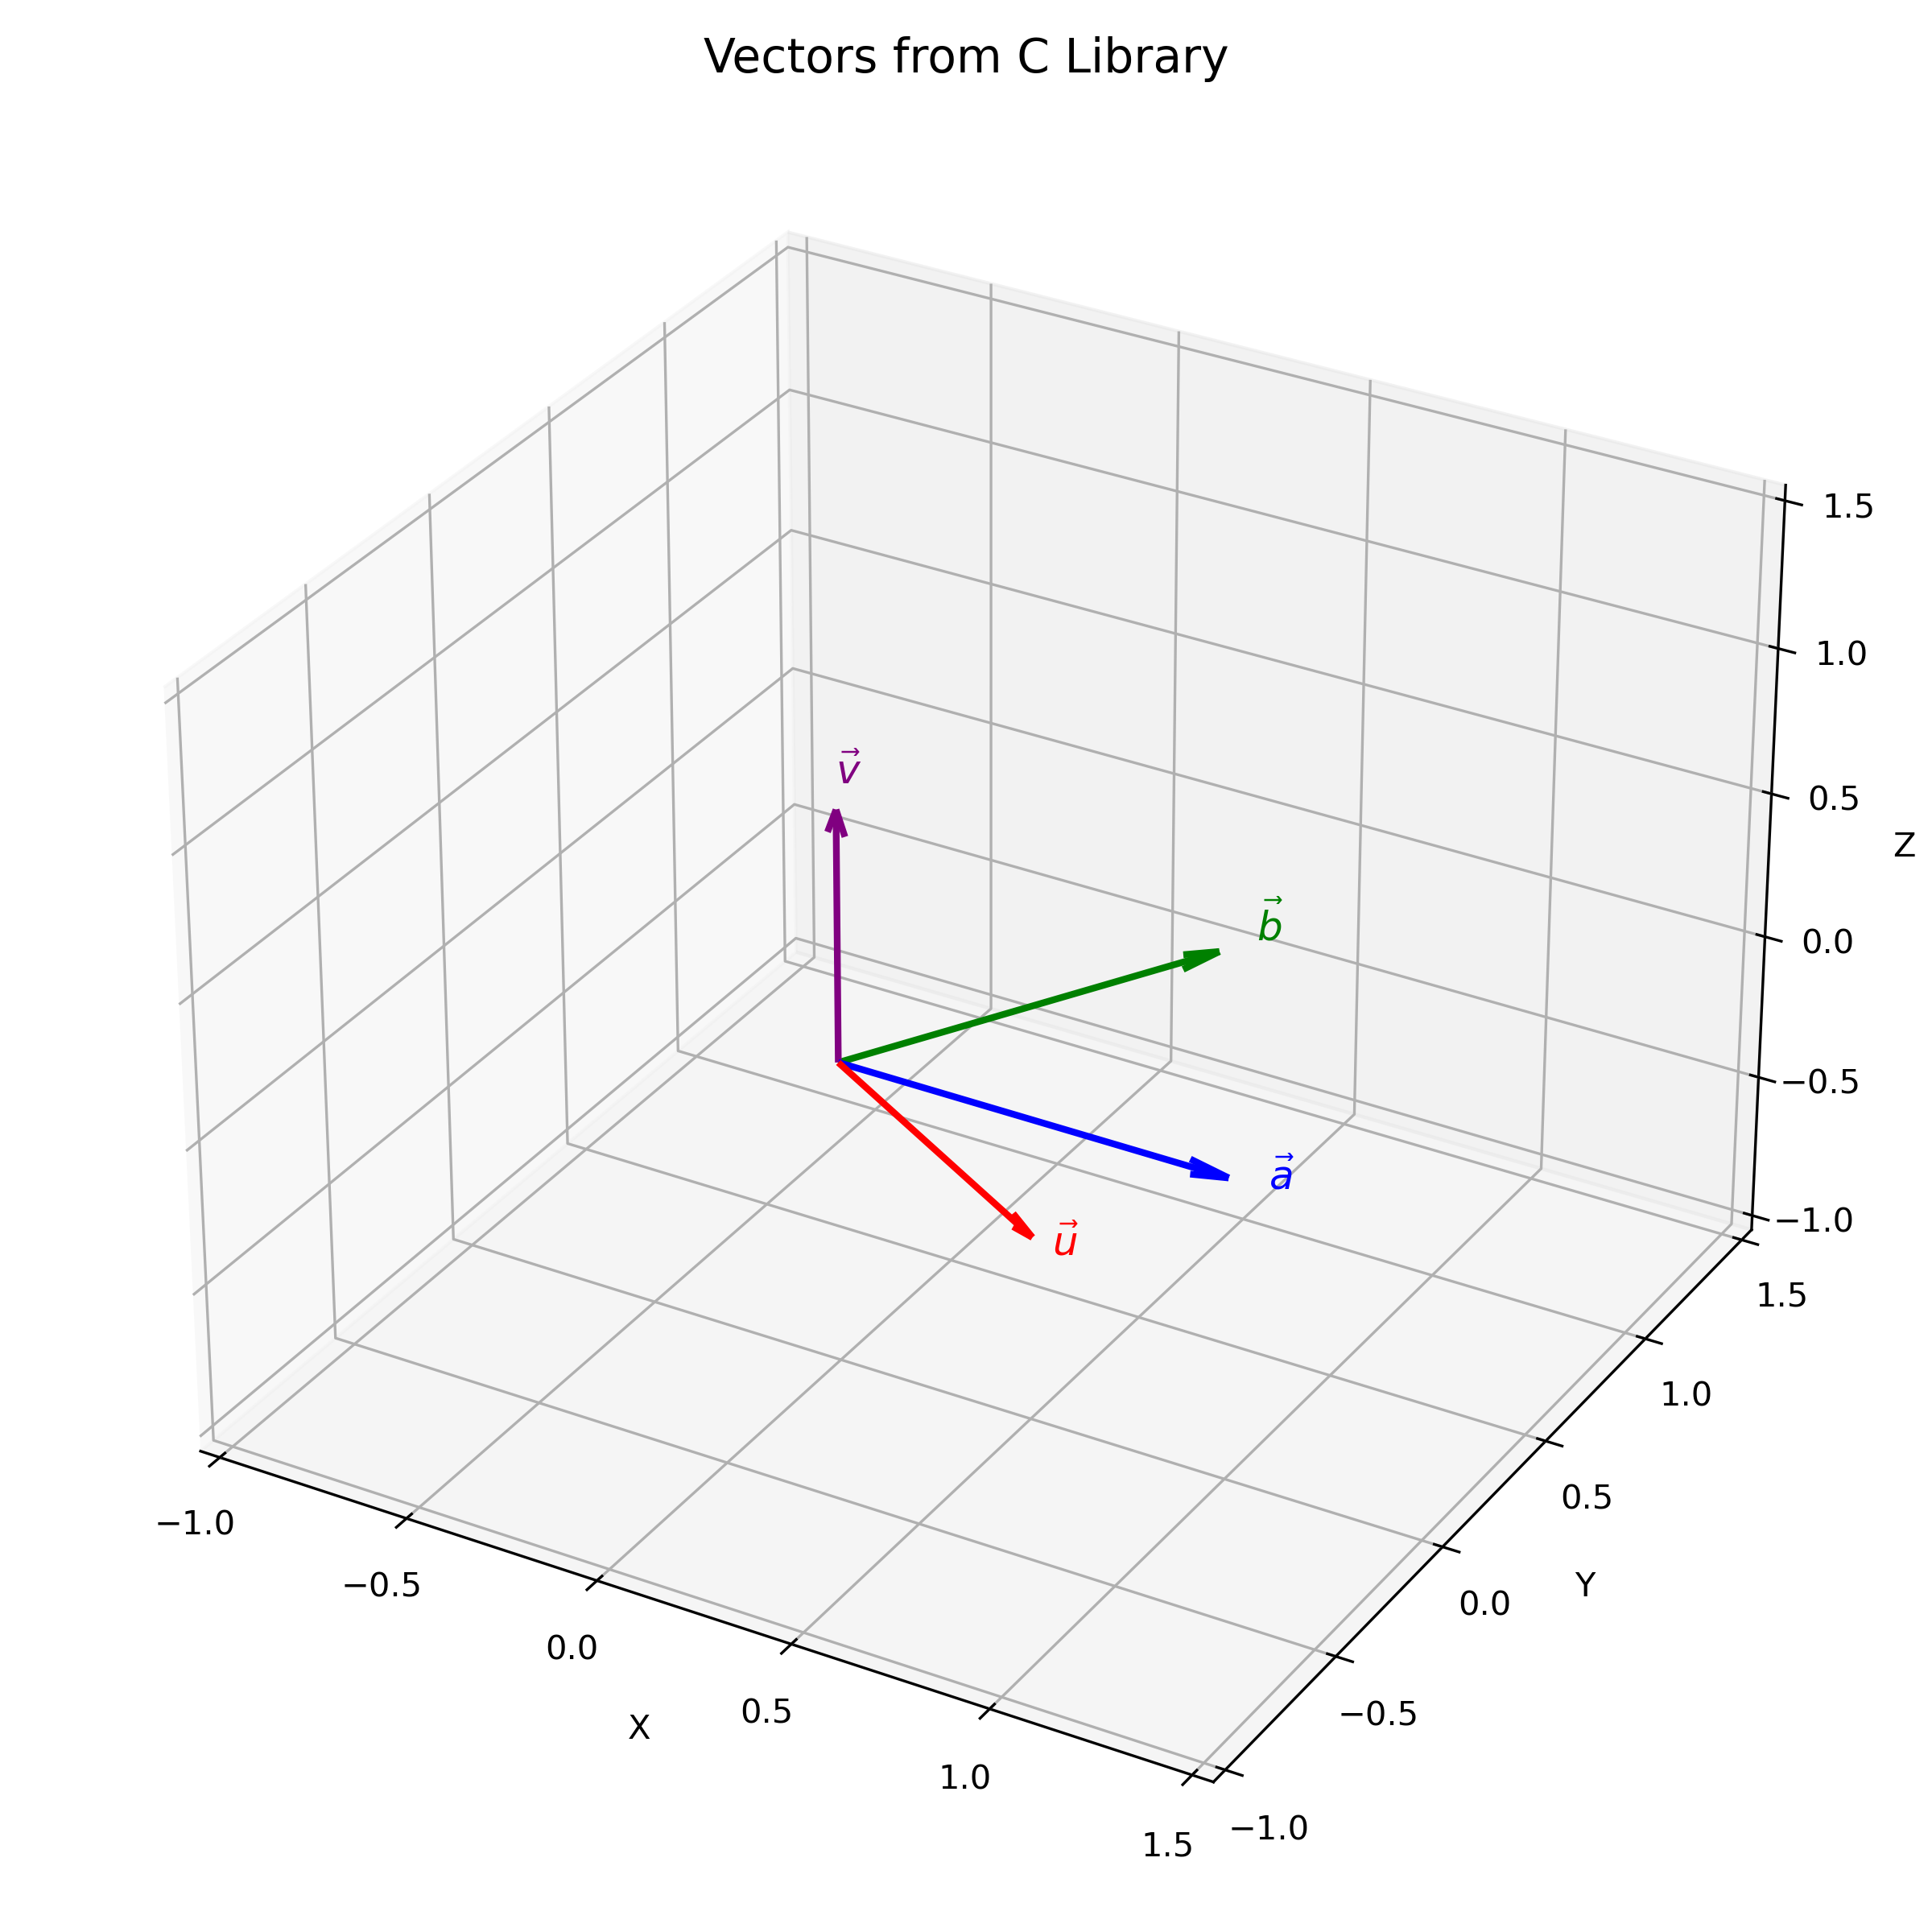
\includegraphics[width=0.6\columnwidth]{figs/vector_plot.png}
   \end{figure}
\end{frame}

\begin{frame}[fragile]
    \frametitle{Code - C}
    \begin{lstlisting}

#include <stdio.h>

// Function to compute dot product
double dot(double a[3], double b[3]) {
    return a[0]*b[0] + a[1]*b[1] + a[2]*b[2];
}

// Function to compute cross product
void cross(double a[3], double b[3], double res[3]) {
    res[0] = a[1]*b[2] - a[2]*b[1];
    res[1] = a[2]*b[0] - a[0]*b[2];
    res[2] = a[0]*b[1] - a[1]*b[0];
}
\end{lstlisting}
\end{frame}

\begin{frame}[fragile]
\frametitle{Code - C}
\begin{lstlisting}

// Function to compute u = a - (a.b)b
void compute_u(double a[3], double b[3], double u[3]) {
    double c = dot(a, b);
    for(int i=0;i<3;i++)
        u[i] = a[i] - c*b[i];
}



\end{lstlisting}
\end{frame}

\begin{frame}[fragile]
    \frametitle{Code - Python(with shared C code)}
    The code to obtain the required plot is
    \begin{lstlisting}
import ctypes
import numpy as np
import matplotlib.pyplot as plt

# Load shared library (Linux/Mac)
lib = ctypes.CDLL("./libvector.so")

# Set argument and return types
lib.compute_u.argtypes = [ctypes.POINTER(ctypes.c_double),
                          ctypes.POINTER(ctypes.c_double),
                          ctypes.POINTER(ctypes.c_double)]
lib.cross.argtypes = [ctypes.POINTER(ctypes.c_double),
                      ctypes.POINTER(ctypes.c_double),
                      ctypes.POINTER(ctypes.c_double)]


\end{lstlisting}
\end{frame}
\begin{frame}[fragile]
\frametitle{Code - Python(with shared C code)}
\begin{lstlisting}
# Helper function to call C compute_u
def compute_u(a, b):
    a_c = (ctypes.c_double * 3)(*a)
    b_c = (ctypes.c_double * 3)(*b)
    u_c = (ctypes.c_double * 3)()
    lib.compute_u(a_c, b_c, u_c)
    return np.array([u_c[0], u_c[1], u_c[2]])

# Helper function to call C cross
def compute_cross(a, b):
    a_c = (ctypes.c_double * 3)(*a)
    b_c = (ctypes.c_double * 3)(*b)
    v_c = (ctypes.c_double * 3)()
    lib.cross(a_c, b_c, v_c)
    return np.array([v_c[0], v_c[1], v_c[2]])

\end{lstlisting}
\end{frame}

\begin{frame}[fragile]
\frametitle{Code - Python(with shared C code)}
\begin{lstlisting}
# Define vectors
a = np.array([1, 0, 0], dtype=float)
b = np.array([0.5, np.sqrt(3)/2, 0], dtype=float)

# Compute using C functions
u = compute_u(a, b)
v = compute_cross(a, b)

print("u =", u)
print("v =", v)

# Plot results
fig = plt.figure(figsize=(8, 8))
ax = fig.add_subplot(111, projection="3d")

\end{lstlisting}
\end{frame}

\begin{frame}[fragile]
\frametitle{Code - Python(with shared C code)}
\begin{lstlisting}
def draw_vec(ax, vec, color, label):
    ax.quiver(0, 0, 0, vec[0], vec[1], vec[2],
              color=color, arrow_length_ratio=0.1, linewidth=2)
    ax.text(vec[0]*1.1, vec[1]*1.1, vec[2]*1.1, label, color=color, fontsize=12)

draw_vec(ax, a, "blue", r"$\vec{a}$")
draw_vec(ax, b, "green", r"$\vec{b}$")
draw_vec(ax, u, "red", r"$\vec{u}$")
draw_vec(ax, v, "purple", r"$\vec{v}$")

ax.set_xlim([-1, 1.5])
ax.set_ylim([-1, 1.5])
ax.set_zlim([-1, 1.5])

\end{lstlisting}
\end{frame}

\begin{frame}[fragile]
\frametitle{Code - Python(with shared C code)}
\begin{lstlisting}

ax.set_xlabel("X")
ax.set_ylabel("Y")
ax.set_zlabel("Z")
ax.set_title("Vectors from C Library", fontsize=14)

plt.tight_layout()

# Save figure to file
plt.savefig("vector_plot.png", dpi=300) 
plt.show()


\end{lstlisting}
\end{frame}

\begin{frame}[fragile]
\frametitle{Code - Python only}
\begin{lstlisting}
import matplotlib.pyplot as plt
import numpy as np

# Define vectors
a = np.array([1, 0, 0])
b = np.array([0.5, np.sqrt(3)/2, 0])

# Compute u = a - (a.b)b
u = a - np.dot(a, b) * b

# Compute v = a x b
v = np.cross(a, b)

print("a =", a)
print("b =", b)
print("u =", u)
print("v =", v)
\end{lstlisting}
\end{frame}
\begin{frame}[fragile]
\frametitle{Code - Python only}
\begin{lstlisting}
# ================== 3D Plot ==================
fig = plt.figure(figsize=(8, 8))
ax = fig.add_subplot(111, projection='3d')

def draw_vec(ax, vec, color, label):
    ax.quiver(0, 0, 0, vec[0], vec[1], vec[2],
              color=color, arrow_length_ratio=0.1, linewidth=2)
    ax.text(vec[0]*1.1, vec[1]*1.1, vec[2]*1.1,
            label, color=color, fontsize=12)

# Draw vectors
draw_vec(ax, a, "blue", r"$\vec{a}$")
draw_vec(ax, b, "green", r"$\vec{b}$")
draw_vec(ax, u, "red", r"$\vec{u}$")
draw_vec(ax, v, "purple", r"$\vec{v}$")




\end{lstlisting}
\end{frame}

\begin{frame}[fragile]
\frametitle{Code - Python only}
\begin{lstlisting}
# Set limits
ax.set_xlim([-1, 1.5])
ax.set_ylim([-1, 1.5])
ax.set_zlim([-1, 1.5])

# Labels
ax.set_xlabel("X")
ax.set_ylabel("Y")
ax.set_zlabel("Z")
ax.set_title("3D Vectors a, b, u, v", fontsize=14)

plt.tight_layout()

# Save figure
plt.savefig("vector_plot_3D.png", dpi=300)
plt.show()

\end{lstlisting}
\end{frame}

\end{document}
